\documentclass[11pt]{article}
\usepackage[T1]{fontenc}
\usepackage[margin=0.85in]{geometry}
\usepackage{graphicx}
\usepackage{xcolor}
\usepackage{listings}
\usepackage{booktabs}
\usepackage{hyperref}
\definecolor{codeblue}{RGB}{36,83,150}
\definecolor{codestring}{RGB}{145,50,45}
\definecolor{codegreen}{RGB}{45,115,75}
\definecolor{codegray}{RGB}{100,100,100}
\lstdefinestyle{python}{
  language=Python,
  basicstyle=\ttfamily\small,
  keywordstyle=\color{codeblue}\bfseries,
  stringstyle=\color{codestring},
  commentstyle=\color{codegreen}\itshape,
  numberstyle=\scriptsize\color{codegray},
  numbers=left,
  numbersep=8pt,
  showstringspaces=false,
  breaklines=true,
  frame=single,
  rulecolor=\color{black!20},
  columns=fullflexible,
  keepspaces=true,
  upquote=true,
  tabsize=4
}
\lstset{style=python}
\hypersetup{colorlinks=true,linkcolor=blue!50!black,urlcolor=blue!50!black}
\title{Bullish News and Bubble Behavior in a Multiround Asset Market\\\large EDSL shared-state pilot}
\author{EDSL replication study}
\date{October 10, 2026}

\begin{document}
\maketitle

\begin{abstract}
This follow-up changes two features of the generic-prompt pilot: all 12 traders
receive explicit behavioral trading instructions, and six receive a strongly
bullish private analyst forecast after period 15. Four participants are
momentum buyers, four are bubble riders, and four are profit-taking sellers.
The one completed 30-period session produced 22 shares traded. Prices rose from
\$15.25 in period 1 to \$17.90 in period 4, then trading paused until periods
27--29, when prices were \$17.75--\$18.00. The prompt design elicited active,
two-sided orders and a brief early price run-up, but the long no-trade interval
means this is not evidence of a sustained bubble or a causal news effect. This
note documents the treatment, shared-state machine, workflow, and results.
\end{abstract}

\section{Design}
The 30-period call market uses 12 traders, each starting with \$100 cash and
four shares. Cash earns 5\% interest; per-share dividends are \$0.40 or \$1.00
with equal probability; the exchange clears a uniform marginal-midpoint price;
and remaining shares are redeemed for \$14 after period 30. The shared public
tape reports prices, volume, and dividends. Traders see their account, personal
history, and the public tape.

All participants receive one of three behavioral prompts: four momentum buyers,
four bubble riders, and four profit-taking sellers. Opening instructions name
concrete limit-price ranges and quantities. This is intended to create buyers
and sellers from the opening periods rather than relying on spontaneous
coordination by identical generic traders.

After period 15 settles, two traders in each behavioral group receive a
private bullish analyst update. The report forecasts that resale prices could
reach \$20 by period 25 because institutional demand is unusually strong. It is
described as a forecast rather than a guaranteed payoff; dividends and actual
terminal redemption remain unchanged. Seed 141027 fixes the behavior composition
and stratified assignment. Recipients: trader-00, trader-01 (momentum);
trader-04, trader-05 (bubble riders); trader-09, trader-11 (profit takers).

\section{Results}
\begin{center}
\begin{tabular}{lr}
\toprule
Measure & Pilot result \\
\midrule
Trader decisions & 360 \\
Settlements & 30 / 30 \\
Private update deliveries & 6 \\
Completed workflow items & 396 / 396 \\
Shares traded & 22 \\
Periods with trade & 7 / 30 \\
Peak observed transaction price & \$18.00 \\
Terminal shares & 0 for every trader \\
Terminal cash range & \$642.76--\$717.52 \\
\bottomrule
\end{tabular}
\end{center}

Transactions occurred in periods 1--4 and 27--29. Prices in the opening
sequence were \$15.25, \$16.63, \$17.25, and \$17.90. The late sequence was \$18.00,
\$17.75, and \$17.75. No transactions occurred in periods 5--26. Across all
decisions, participants submitted 181 buy orders and 39 sell orders. Momentum
traders submitted 78 buys; bubble riders submitted 103 buys; profit takers
submitted 15 sells. Many orders did not fill, so these counts describe intended
orders rather than completed trades.

The mean current-price forecast for update recipients was \$17.77 in period 15,
\$17.93 in period 16, and \$18.17 in period 25. For traders without the update,
the corresponding means were \$17.77, \$17.77, and \$17.90. This small descriptive
gap is consistent with some response to the news, but it is not a causal
estimate. Traders share a market, and there is only one session.

\begin{figure}[ht]
\centering
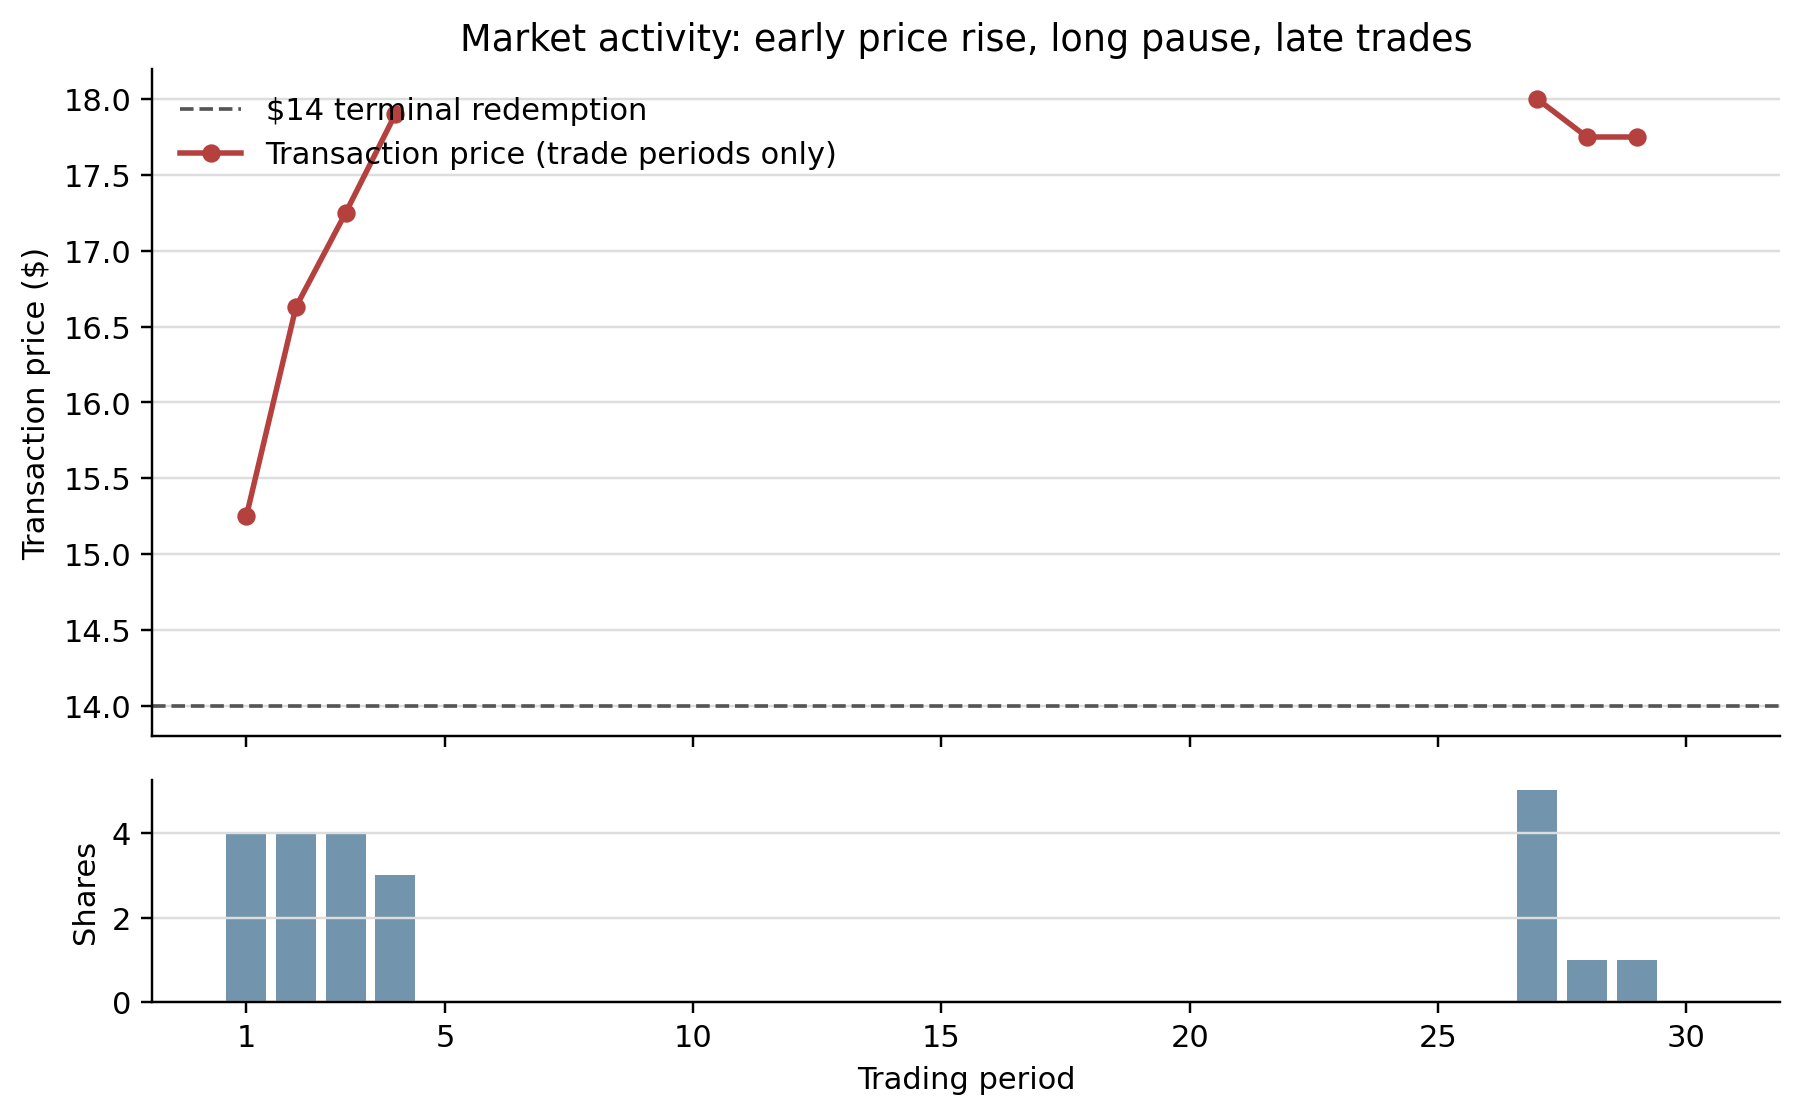
\includegraphics[width=0.88\linewidth]{market_outcomes.png}
\caption{Observed transaction prices and traded volume. The \$14 line is the
terminal redemption amount. Missing price points indicate periods with no
transaction.}
\end{figure}

\begin{figure}[ht]
\centering
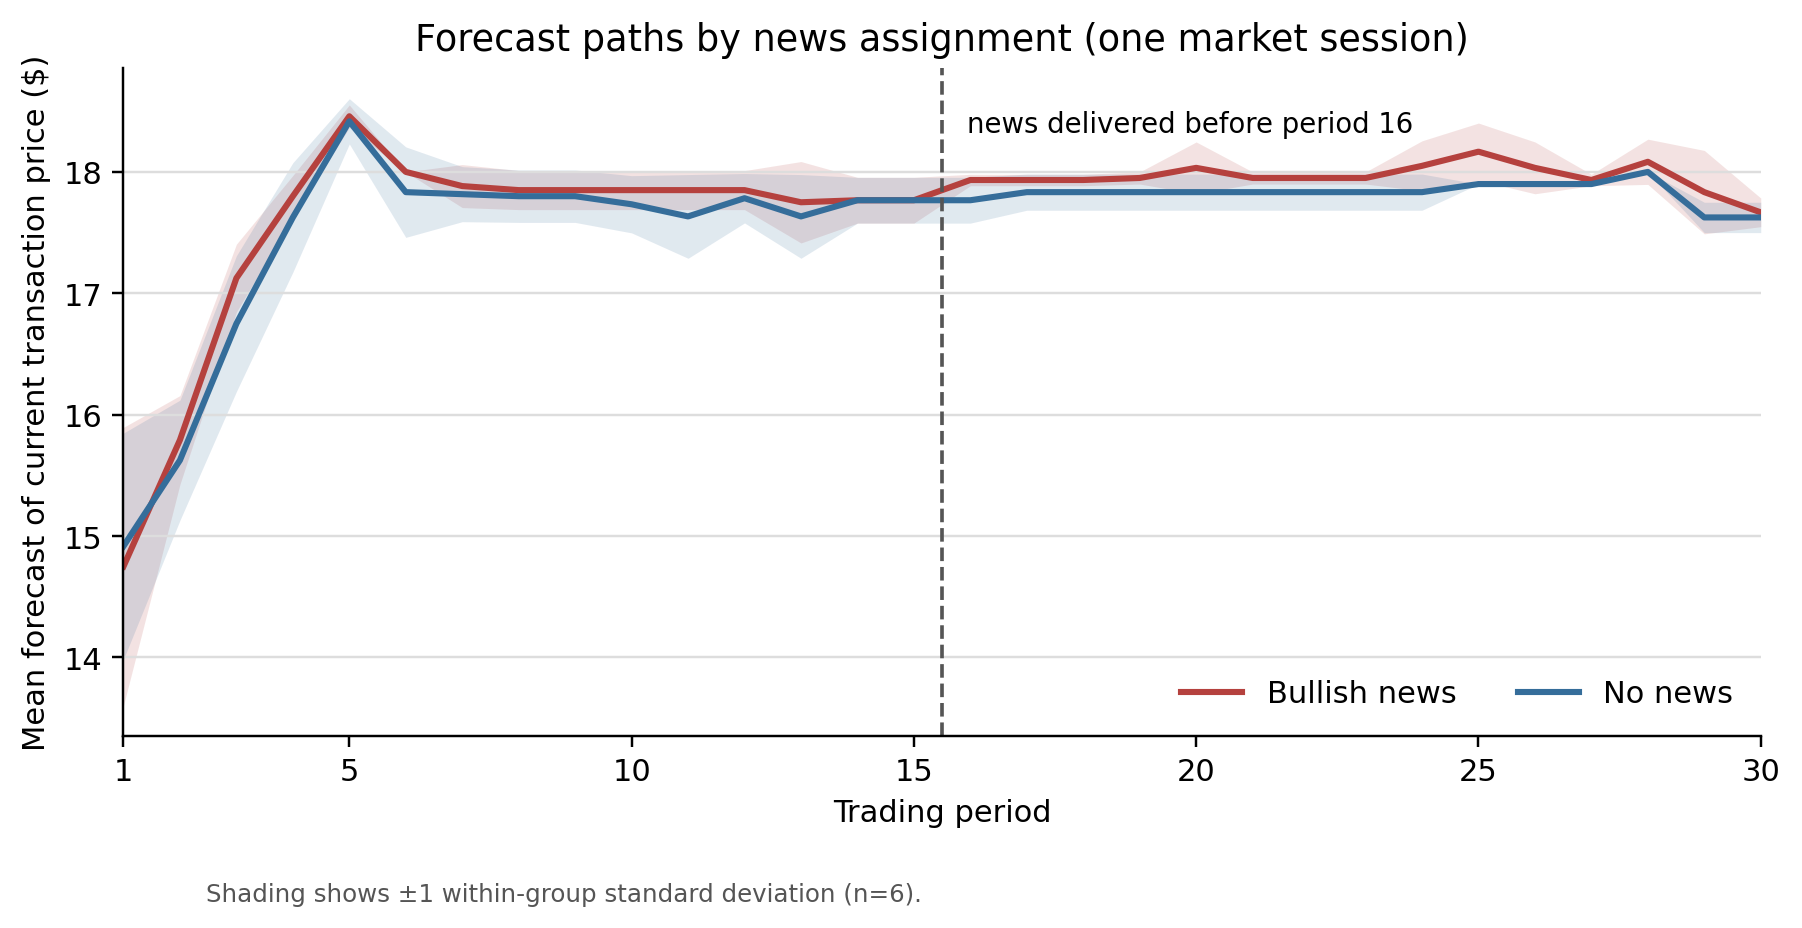
\includegraphics[width=0.88\linewidth]{forecast_paths.png}
\caption{Mean current-price forecasts by update assignment. Shading is one
within-group standard deviation ($n=6$), not a confidence interval. The update
was delivered before period 16.}
\end{figure}

The prompts produced a brief opening run-up above the terminal redemption
amount, followed by 22 inactive periods and three late trading periods. The
result is a useful pilot for a bubble-inducing instruction set, not a sustained
bubble. The next evidence should come from multiple independently seeded
markets, preferably with enough sessions to estimate variation across market
composition and treatment assignment.

\clearpage
\section{Shared-state machine}
The experiment starts from EDSL's native `call\_market` machine, which defines
accounts, orders, order history, tape, period, last price, settlement, interest,
dividends, and redemption. It adds a private update map and one command. The
machine's public view includes the trader's account and shared tape; the added
projection selects only the update for the current trader.

\begin{lstlisting}
machine = call_market(TRADERS, rules=RULES, seed=SEED)
machine.fields["private_updates"] = state_field(StateType.map(), {})
machine.commands["publish_update"] = Command(
    inputs={"recipient": StateType.text(), "message": StateType.text()},
    effects=(put("private_updates", arg("recipient"), arg("message")),),
)
machine.view["your_update"] = field("private_updates").get(current("name"))
machine.validate()
\end{lstlisting}

The private map itself is not present in the trader-facing view. The DSL lookup
uses the current participant's name to select one entry and yields an update
only to that participant. Everyone else gets
an empty result rendered as “No private analyst update has been issued to you.”
Each publication is a separate workflow write, so recipient, message, and event
order are persisted and auditable.

\begin{figure}[ht]
\centering
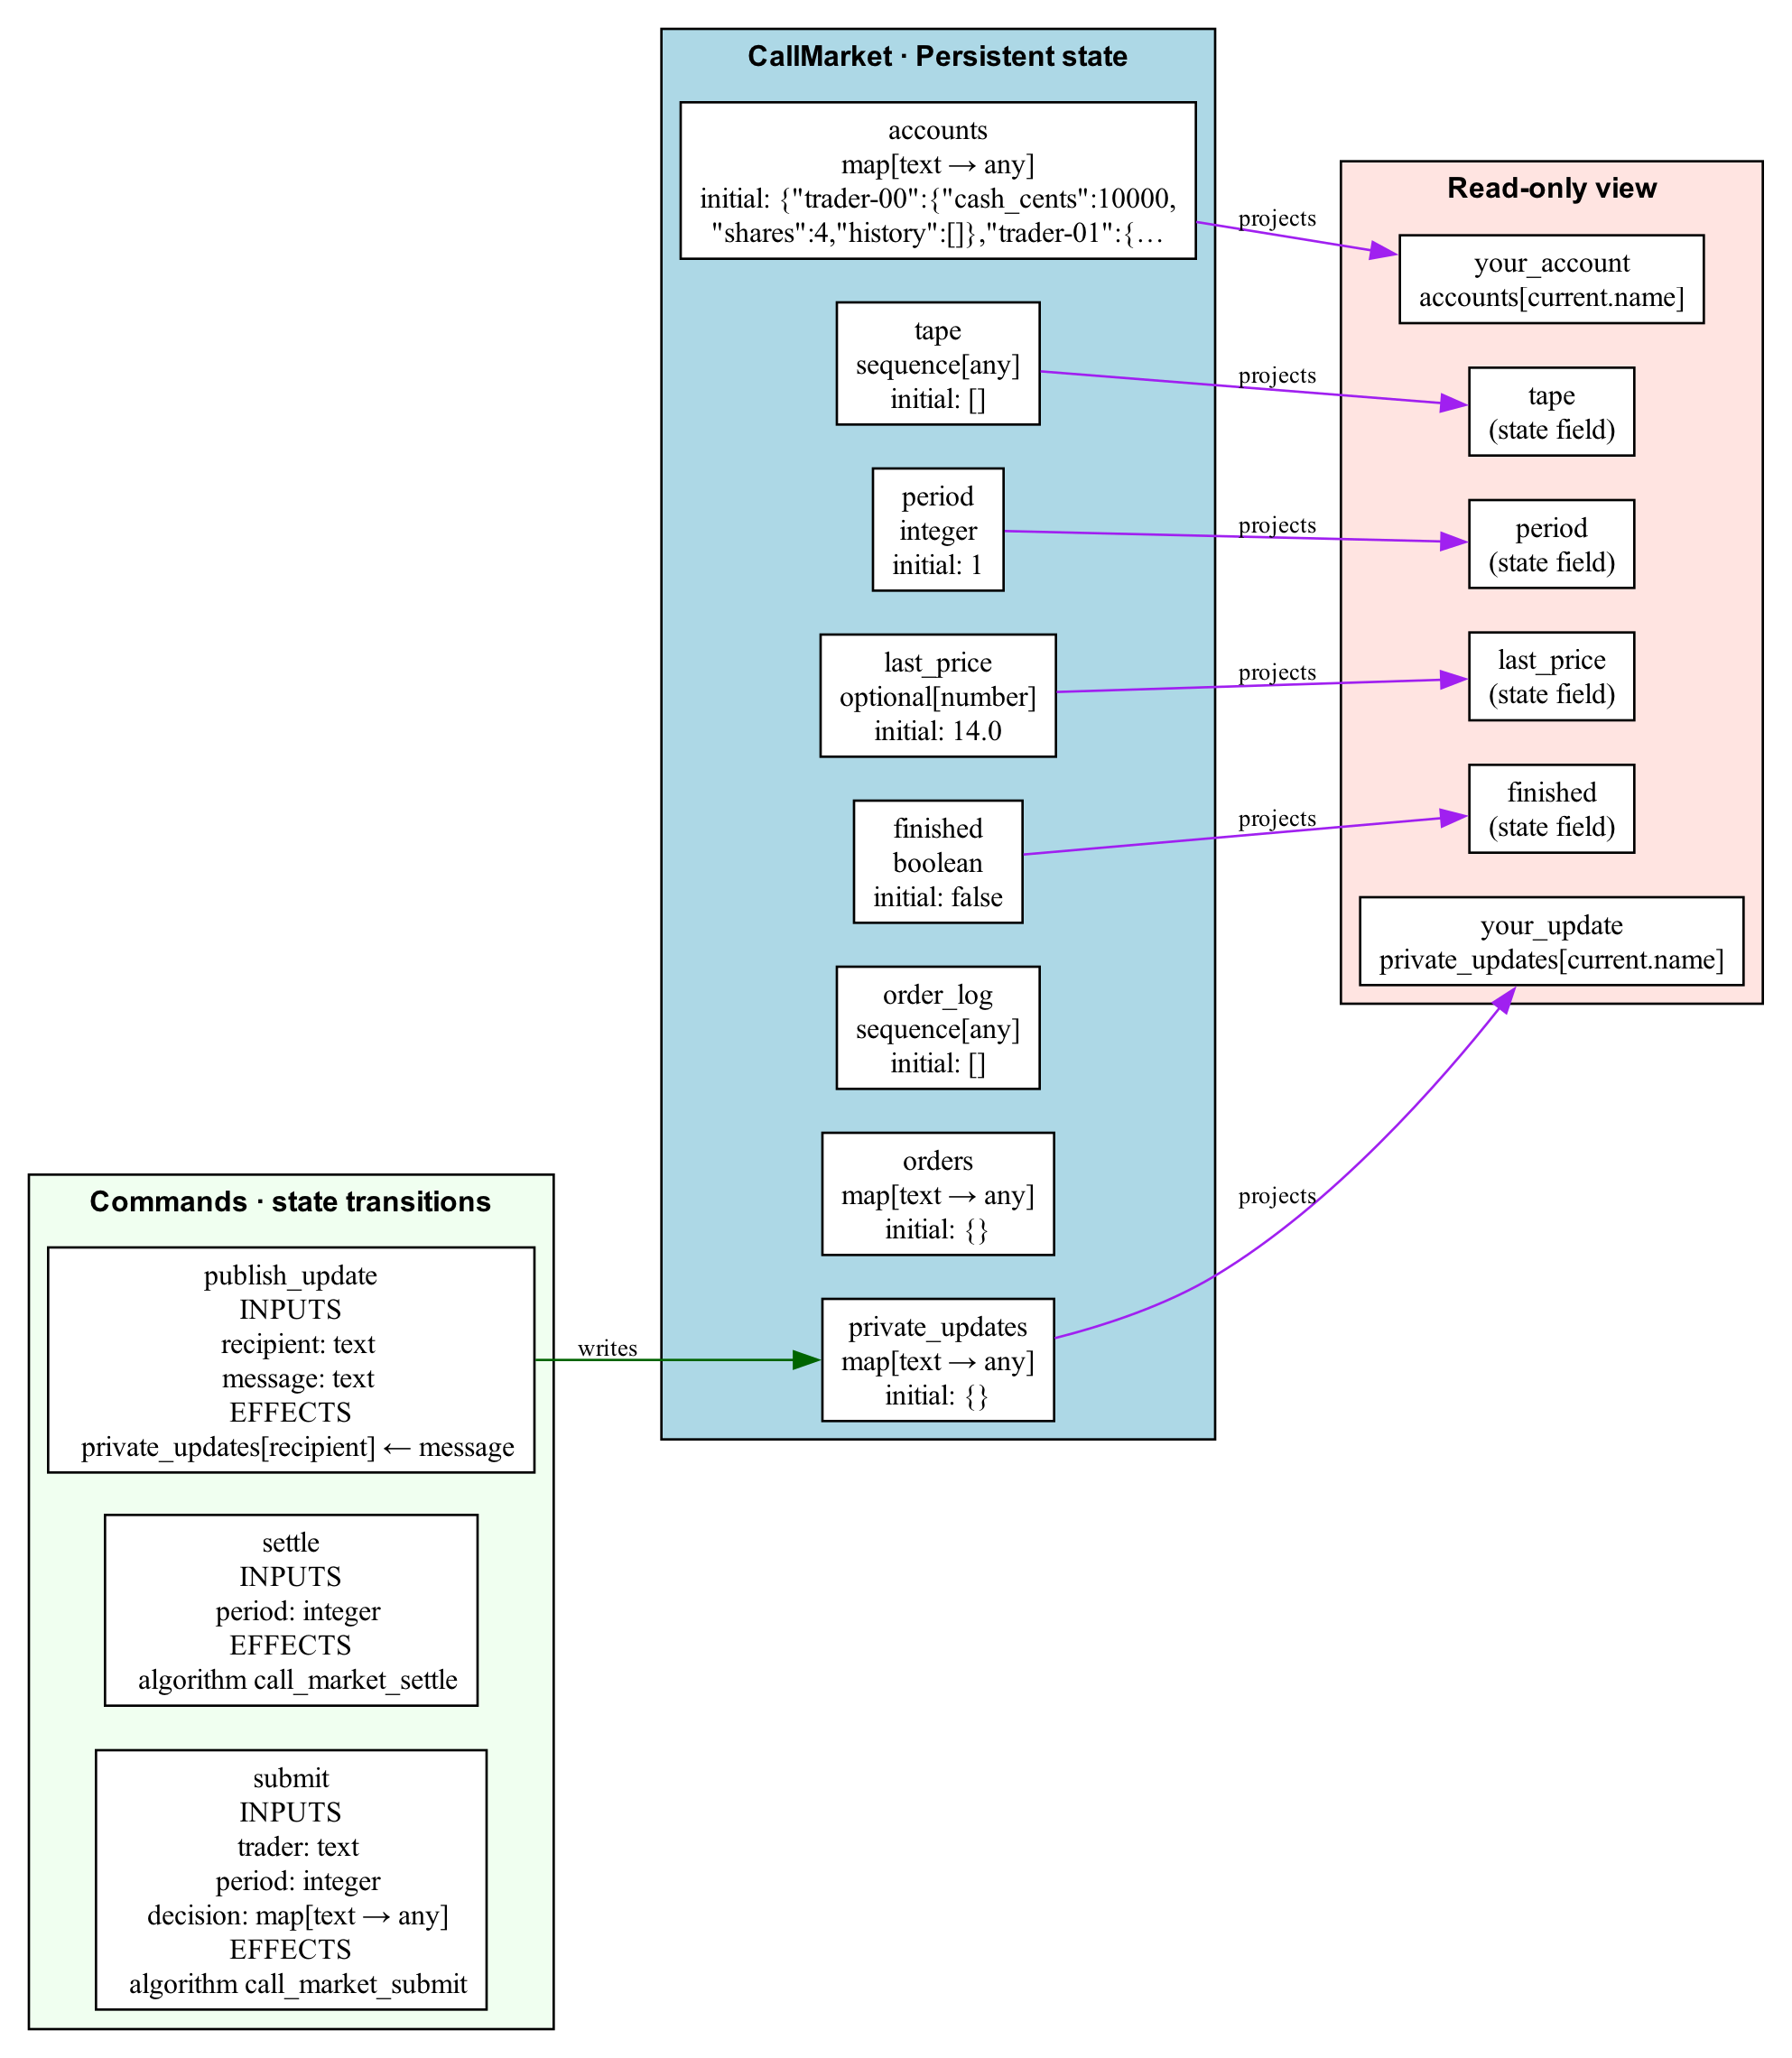
\includegraphics[width=0.62\linewidth,height=0.75\textheight,keepaspectratio]{market_machine.png}
\caption{Detailed diagram generated by EDSL's `Machine.show\_diagram` method.}
\end{figure}

\section{Round execution and midpoint update}
Each period consists of a trader order step followed by exchange settlement.
Trader work reads the machine and writes each structured decision through
`submit`; settlement calls the native deterministic market algorithm. After
period 15 settlement, six scripted exchange items publish the updates in a
chain. Period 16 trader work waits for all six writes, so the message is absent
from earlier views and available in the intended recipients' next decisions.

\begin{lstlisting}
orders = workflow.step(
    f"orders-{period}", Survey([decision]),
    assigned_to=role("trader"), after=previous,
    reads=(market.read(),),
    writes=(market.submit(
        trader=current.agent.name, period=period,
        decision=decision.answer,
    ),),
)
settled = workflow.step(
    f"settle-{period}", settlement_survey,
    assigned_to=role("exchange"), after=orders,
    writes=(market.settle(period=period),),
)
previous = settled
if period == 15:
    for recipient in recipients:
        previous = workflow.step(
            f"publish-private-update-{recipient}", update_survey,
            assigned_to=role("exchange"), after=previous,
            writes=(market.publish_update(
                recipient=recipient, message=UPDATE,
            ),),
        )
\end{lstlisting}

The six update tasks use a scripted exchange answer, so they create no model
calls. The trader behavior is stored in each agent's traits and supplied as
behavioral instructions at every decision period. Treatment status is a
separate trait and does not replace the behavior persona.

\section{Run command}
Preparation writes the serializable experiment and machine without inference:

\begin{lstlisting}
python3 edsl_replication/studies/asset_market_bullish_bubble/experiment.py \
  --output edsl_replication/studies/asset_market_bullish_bubble/pilot_01 \
  --prepare-only
\end{lstlisting}

The pilot was launched locally through EDSL using the configured provider
credentials, with `--prepare-only` omitted. EDSL wrote its workflow database,
shared-state SQLite log, model calls, and job artifacts under `pilot\_01/`.

\section{Limits}
This is one market with a mixed treatment and one common tape. Information can
spread through observed behavior and transaction prices, so traders are not
independent experimental units. The strongly positive analyst forecast is
belief-relevant but does not change realized dividend or redemption rules. The
22 shares traded and short opening price run-up motivate replications; they do
not establish a bubble or the causal effect of news or behavioral prompts.

\end{document}
